\section{Tiny turtle graphics
interpreter}\label{tiny-turtle-graphics-interpreter}

A program \passthrough{\lstinline!turtle!} is an example with the
combination of TfeTextView and GtkDrawingArea objects. It is a very
small interpreter but you can draw fractal curves with it. The following
diagram is a Koch curve, which is one of the famous fractal curves.

\begin{figure}
\centering
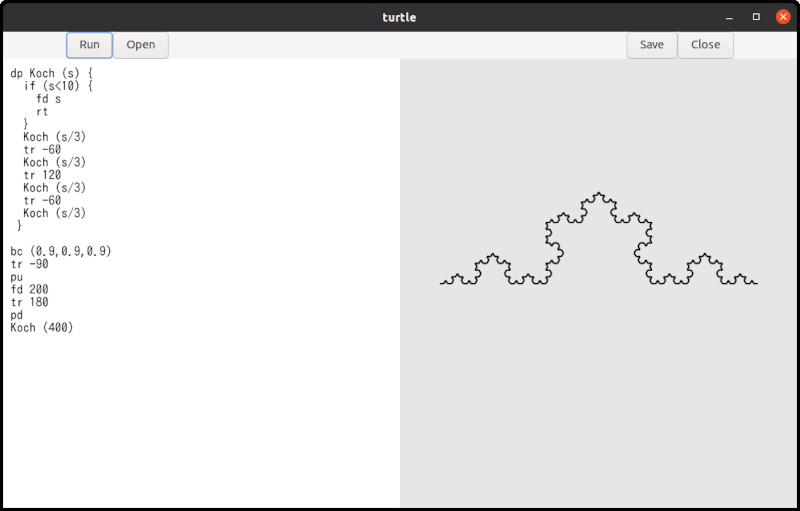
\includegraphics[width=8cm,height=5.11cm]{../src/turtle/image/turtle_koch.png}
\caption{Koch curve}
\end{figure}

The following is a snow-crystal-shaped curve. It is composed of six Koch
curves.

\begin{figure}
\centering
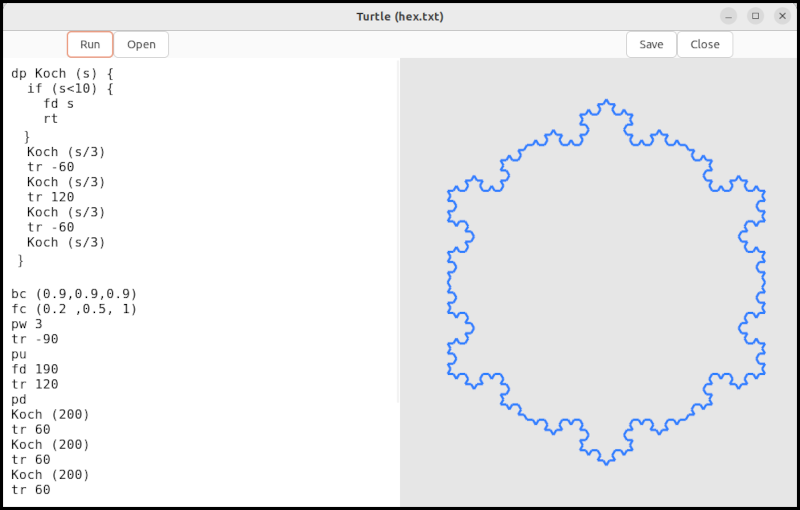
\includegraphics[width=8cm,height=5.11cm]{../image/turtle_snow.png}
\caption{Snow}
\end{figure}

This program uses flex and bison. Flex is a lexical analyzer. Bison is a
parser generator. These two programs are similar to lex and yacc which
are proprietary software developed in Bell Laboratory. However, flex and
bison are open source software. This section describes them and they are
not the topics about GTK 4. So, readers can skip this section.

\subsection{How to use turtle}\label{how-to-use-turtle}

The turtle document is in the appendix. I'll show you a simple example.

\begin{lstlisting}
fc (1,0,0) # Foreground color is red, rgb = (1,0,0).
pd         # Pen down.
rp (4) {   # Repeat four times.
  fd 100   # Go forward by 100 pixels.
  tr 90    # Turn right by 90 degrees.
}
\end{lstlisting}

\begin{enumerate}
\def\labelenumi{\arabic{enumi}.}
\tightlist
\item
  Compile and install \passthrough{\lstinline!turtle!} (See the
  documentation above). Then, run \passthrough{\lstinline!turtle!}.
\item
  Type the program above in the editor (left part of the window).
\item
  Click on the \passthrough{\lstinline!Run!} button, then a red square
  appears on the right part of the window. The side of the square is 100
  pixels long.
\end{enumerate}

In the same way, you can draw other curves. The turtle document includes
some fractal curves such as tree, snow and square-koch. The source codes
are located at src/turtle/example directory. You can read these files
into \passthrough{\lstinline!turtle!} editor by clicking on the
\passthrough{\lstinline!Open!} button.

\subsection{Combination of TfeTextView and GtkDrawingArea
objects}\label{combination-of-tfetextview-and-gtkdrawingarea-objects}

Turtle uses TfeTextView and GtkDrawingArea.

\begin{enumerate}
\def\labelenumi{\arabic{enumi}.}
\tightlist
\item
  A user inputs/reads a turtle program into the buffer in the
  TfeTextView instance.
\item
  The user clicks on the ``Run'' button.
\item
  The parser reads the program and generates tree-structured data.
\item
  The interpriter reads the data and executes it step by step. And it
  draws shapes on a surface. The surface isn't the one in the
  GtkDrawingArea widget.
\item
  The widget is added to the queue. It will be redrawn with the drawing
  function, which just copies the surface into the one in the
  GtkDrawingArea.
\end{enumerate}

\begin{figure}
\centering
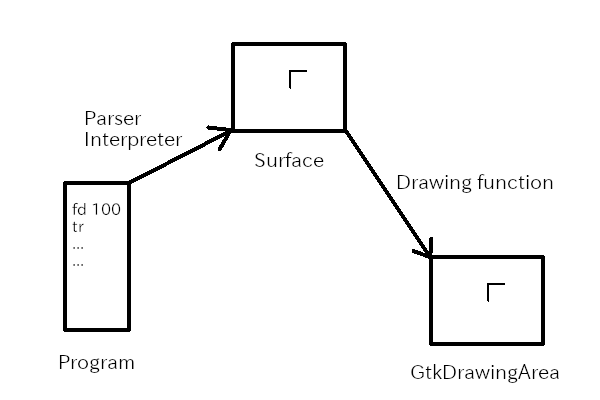
\includegraphics{../image/turtle.png}
\caption{Parser, interpreter and drawing function}
\end{figure}

The body of the interpreter is written with flex and bison. The codes
are not thread safe. So the callback function
\passthrough{\lstinline!run\_cb!}, which is the handler of ``clicked''
signal on the \passthrough{\lstinline!Run!} button, prevents reentering.

\begin{lstlisting}[language=C, numbers=left]
void
run_cb (GtkWidget *btnr) {
  GtkTextBuffer *tb = gtk_text_view_get_buffer (GTK_TEXT_VIEW (tv));
  GtkTextIter start_iter;
  GtkTextIter end_iter;
  char *contents;
  int stat;
  static gboolean busy = FALSE; /* initialized only once */
  cairo_t *cr;

  /* yyparse() and run() are NOT thread safe. */
  /* The variable busy avoids reentrance. */
  if (busy)
    return;
  busy = TRUE;
  gtk_text_buffer_get_bounds (tb, &start_iter, &end_iter);
  contents = gtk_text_buffer_get_text (tb, &start_iter, &end_iter, FALSE);
  if (surface && contents[0] != '\0') {
    init_flex (contents);
    stat = yyparse ();
    if (stat == 0) { /* No error */
      run ();
    }
    finalize_flex ();
  } else if (surface) {
    cr = cairo_create (surface);
    cairo_set_source_rgb (cr, 1.0, 1.0, 1.0);
    cairo_paint (cr);
    cairo_destroy (cr);
  }
  g_free (contents);
  gtk_widget_queue_draw (GTK_WIDGET (da));
  busy = FALSE;
}

static void
resize_cb (GtkDrawingArea *drawing_area, int width, int height, gpointer user_data) {

  if (surface)
    cairo_surface_destroy (surface);
  surface = cairo_image_surface_create (CAIRO_FORMAT_ARGB32, width, height);
  run_cb (NULL); // NULL is a fake (run button).
}
\end{lstlisting}

\begin{itemize}
\tightlist
\item
  8, 13-15: The static value \passthrough{\lstinline!busy!} holds a
  status of the interpreter. If it is \passthrough{\lstinline!TRUE!},
  the interpreter is running and it is not possible to call the
  interpreter because it's not a re-entrant program. If it is
  \passthrough{\lstinline!FALSE!}, it is safe to call the interpreter
  and set the variable \passthrough{\lstinline!busy!} to TRUE.
\item
  16-17: Gets the contents of \passthrough{\lstinline!tb!}.
\item
  18-30: The variable \passthrough{\lstinline!surface!} is a static
  variable. It points to a \passthrough{\lstinline!cairo\_surface\_t!}
  instance. It is created when the GtkDrawingArea instance is realized
  and whenever it is resized. Therefore,
  \passthrough{\lstinline!surface!} isn't NULL usually. But if it is
  NULL, the interpreter won't be called.
\item
  18-24: If \passthrough{\lstinline!surface!} points a surface instance
  and the string \passthrough{\lstinline!contents!} isn't empty, it
  calls the interpreter.

  \begin{itemize}
  \tightlist
  \item
    Initializes the lexical analyzer.
  \item
    Calls the parser. The parser analyzes the program codes
    syntactically and generates a tree structured data.
  \item
    If the parser successfully parsed, it calls the runtime routine
    `run'.
  \item
    Finalizes the lexical analyzer.
  \end{itemize}
\item
  25-29: If \passthrough{\lstinline!surface!} points a surface instance
  and the string \passthrough{\lstinline!contents!} is empty, it clears
  the surface \passthrough{\lstinline!surface!}.
\item
  31: Frees \passthrough{\lstinline!contents!}.
\item
  32: Adds the drawing area widget to the queue to draw.
\item
  33: Sets the variable \passthrough{\lstinline!busy!} to FALSE.
\item
  36-43: The ``resized'' signal handler. If the
  \passthrough{\lstinline!surface!} isn't NULL, it is destroyed. A new
  surface is created. Its size is the same as the surface of the
  GtkDrawingArea instance. It calls the callback function
  \passthrough{\lstinline!run\_cb!} to redraw the shape on the drawing
  area.
\end{itemize}

If the open button is clicked and a file is read, the filename will be
shown on the header bar.

\begin{lstlisting}[language=C, numbers=left]
static void
show_filename (TfeTextView *tv) {
  GFile *file;
  char *filename;
  char *title;

  file = tfe_text_view_get_file (tv);
  if (G_IS_FILE (file)) {
    filename = g_file_get_basename (file);
    title = g_strdup_printf ("Turtle (%s)", filename);
    g_free (filename);
    g_object_unref (file);
  } else
    title = g_strdup ("Turtle");
  gtk_window_set_title (GTK_WINDOW (win), title);
  g_free (title);
}
\end{lstlisting}

This function is the callback function of the ``change-file'' signal on
the TfeTextView instance. It calls
\passthrough{\lstinline!tfe\_text\_view\_get\_file!}.

\begin{itemize}
\tightlist
\item
  If the return value is a GFile instance, the title will be ``Turtle
  (the filename)''.
\item
  Otherwise, the title will be ``Turtle''.
\end{itemize}

Other part of \passthrough{\lstinline!turtleapplication.c!} is very
simple and similar to the codes in the former applications. The codes of
\passthrough{\lstinline!turtleapplication.c!} is in the turtle
directory.

\subsection{What does the interpreter
do?}\label{what-does-the-interpreter-do}

Suppose that the turtle application runs with the following program.

\begin{lstlisting}
distance = 100
fd distance*2
\end{lstlisting}

The application recognizes the program and works as follows.

\begin{itemize}
\tightlist
\item
  Generally, a program consists of tokens. Tokens are ``distance'',
  ``='', ``100'', ``fd'', ``*'' and ``2'' in the above example..
\item
  The parser calls a function \passthrough{\lstinline!yylex!} to read a
  token in the source file. \passthrough{\lstinline!yylex!} returns a
  code which is called ``token kind'' and sets a global variable
  \passthrough{\lstinline!yylval!} to a value, which is called a
  semantic value. The type of \passthrough{\lstinline!yylval!} is union.
  The type of \passthrough{\lstinline!yylval.ID!} and
  \passthrough{\lstinline!yylval.NUM!} are string and double
  respectively. There are seven tokens in the program so
  \passthrough{\lstinline!yylex!} is called seven times.
\end{itemize}

\begin{longtable}[]{@{}cccc@{}}
\toprule\noalign{}
& token kind & yylval.ID & yylval.NUM \\
\midrule\noalign{}
\endhead
\bottomrule\noalign{}
\endlastfoot
1 & ID & distance & \\
2 & = & & \\
3 & NUM & & 100 \\
4 & FD & & \\
5 & ID & distance & \\
6 & * & & \\
7 & NUM & & 2 \\
\end{longtable}

\begin{itemize}
\tightlist
\item
  The function \passthrough{\lstinline!yylex!} returns a token kind
  every time, but it doesn't set \passthrough{\lstinline!yylval.ID!} or
  \passthrough{\lstinline!yylval.NUM!} every time. It is because
  keywords (\passthrough{\lstinline!FD!}) and symbols
  (\passthrough{\lstinline!=!} and \passthrough{\lstinline!*!}) don't
  have any semantic values. The function \passthrough{\lstinline!yylex!}
  is called lexical analyzer or scanner.
\item
  The application \passthrough{\lstinline!turtle!} makes a tree
  structured data. This part of \passthrough{\lstinline!turtle!} is
  called parser.
\end{itemize}

\begin{figure}
\centering
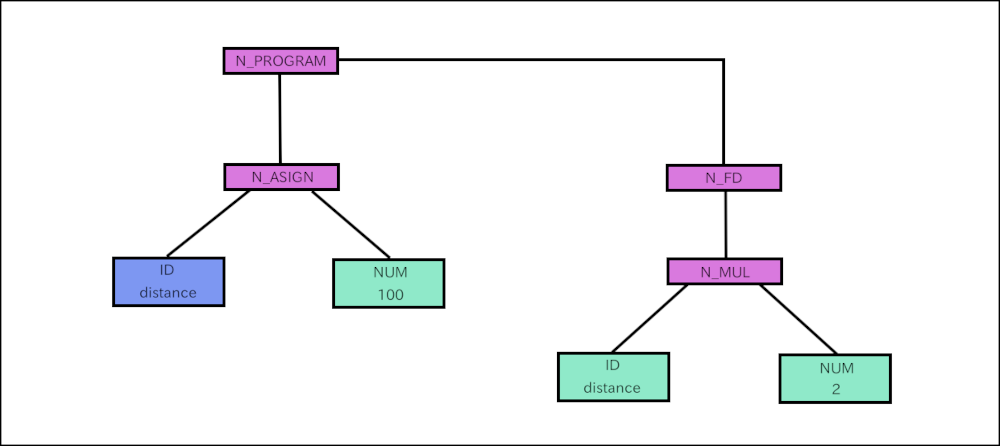
\includegraphics[width=12cm,height=5.34cm]{../image/turtle_parser_tree.png}
\caption{turtle parser tree}
\end{figure}

\begin{itemize}
\tightlist
\item
  \passthrough{\lstinline!Turtle!} analyzes the tree and executes it.
  This part of \passthrough{\lstinline!turtle!} is called runtime
  routine or interpreter. The tree consists of rectangles and line
  segments between the rectangles. The rectangles are called nodes. For
  example, N\_PROGRAM, N\_ASSIGN, N\_FD and N\_MUL are nodes.

  \begin{enumerate}
  \def\labelenumi{\arabic{enumi}.}
  \tightlist
  \item
    Goes down from N\_PROGRAM to N\_ASSIGN.
  \item
    N\_ASSIGN node has two children, ID and NUM. This node comes from
    ``distance = 100'' which is ``ID = NUM'' syntactically. First,
    \passthrough{\lstinline!turtle!} checks if the first child is ID. If
    it's ID, then \passthrough{\lstinline!turtle!} looks for the
    variable in the variable table. If it doesn't exist, it registers
    the ID (\passthrough{\lstinline!distance!}) to the table. Then go
    back to the N\_ASSIGN node.
  \item
    \passthrough{\lstinline!Turtle!} calculates the second child. In
    this case its a number 100. Saves 100 to the variable table at the
    \passthrough{\lstinline!distance!} record.
  \item
    \passthrough{\lstinline!Turtle!} goes back to N\_PROGRAM then go to
    the next node N\_FD. It has only one child. Goes down to the child
    N\_MUL.
  \item
    The first child is ID (distance). Searches the variable table for
    the variable \passthrough{\lstinline!distance!} and gets the value
    100. The second child is a number 2. Multiplies 100 by 2 and gets
    200. Then \passthrough{\lstinline!turtle!} goes back to N\_FD.
  \item
    Now \passthrough{\lstinline!turtle!} knows the distance is 200. It
    moves the cursor forward by 200 pixels. The segment is drawn on the
    \passthrough{\lstinline!surface!}.
  \item
    There are no node follows. Runtime routine returns to the function
    \passthrough{\lstinline!run\_cb!}.
  \end{enumerate}
\item
  The function \passthrough{\lstinline!run\_cb!} calls
  \passthrough{\lstinline!gtk\_widget\_queue\_draw!} and put the
  GtkDrawingArea widget to the queue.
\item
  The system redraws the widget. At that time drawing function
  \passthrough{\lstinline!draw\_func!} is called. The function copies
  the \passthrough{\lstinline!surface!} to the surface in the
  GtkDrawingArea.
\end{itemize}

Actual turtle program is more complicated than the example above.
However, what turtle does is basically the same. Interpretation consists
of three parts.

\begin{itemize}
\tightlist
\item
  Lexical analysis
\item
  Syntax Parsing and tree generation
\item
  Interpretation and execution of the tree.
\end{itemize}

\subsection{Compilation flow}\label{compilation-flow}

The source files are:

\begin{itemize}
\tightlist
\item
  flex source file =\textgreater{} \passthrough{\lstinline!turtle.lex!}
\item
  bison source file =\textgreater{} \passthrough{\lstinline!turtle.y!}
\item
  C header file =\textgreater{} \passthrough{\lstinline!turtle\_lex.h!}
\item
  C source file =\textgreater{}
  \passthrough{\lstinline!turtleapplication.c!}
\item
  other files =\textgreater{} \passthrough{\lstinline!turtle.ui!},
  \passthrough{\lstinline!turtle.gresources.xml!} and
  \passthrough{\lstinline!meson.build!}
\end{itemize}

The compilation process is a bit complicated.

\begin{enumerate}
\def\labelenumi{\arabic{enumi}.}
\tightlist
\item
  glib-compile-resources compiles \passthrough{\lstinline!turtle.ui!} to
  \passthrough{\lstinline!resources.c!} according to
  \passthrough{\lstinline!turtle.gresource.xml!}. It also generates
  \passthrough{\lstinline!resources.h!}.
\item
  bison compiles \passthrough{\lstinline!turtle.y!} to
  \passthrough{\lstinline!turtle\_parser.c!} and generates
  \passthrough{\lstinline!turtle\_parser.h!}
\item
  flex compiles \passthrough{\lstinline!turtle.lex!} to
  \passthrough{\lstinline!turtle\_lex.c!}.
\item
  gcc compiles \passthrough{\lstinline!application.c!},
  \passthrough{\lstinline!resources.c!},
  \passthrough{\lstinline!turtle\_parser.c!} and
  \passthrough{\lstinline!turtle\_lex.c!} with
  \passthrough{\lstinline!turtle\_lex.h!},
  \passthrough{\lstinline!resources.h!} and
  \passthrough{\lstinline!turtle\_parser.h!}. It generates an executable
  file \passthrough{\lstinline!turtle!}.
\end{enumerate}

\begin{figure}
\centering
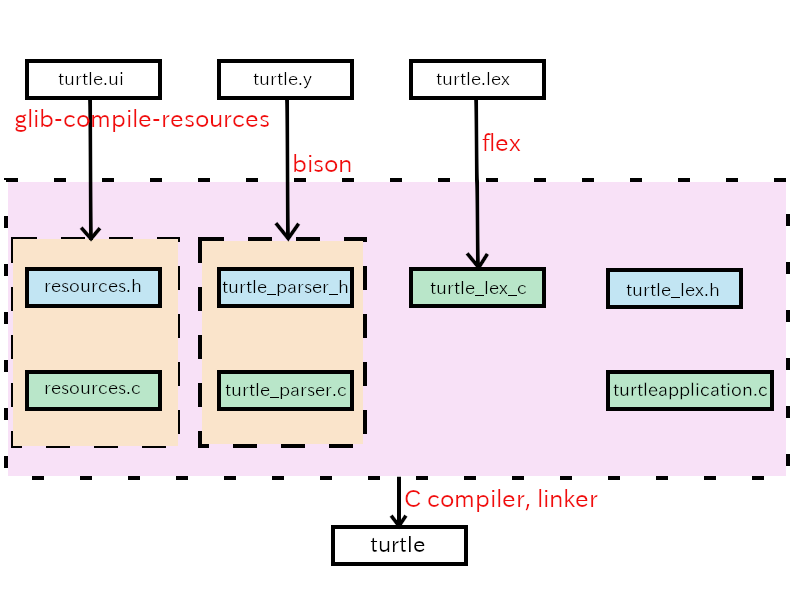
\includegraphics[width=12cm,height=9cm]{../image/turtle_compile_process.png}
\caption{compile process}
\end{figure}

Meson controls the process. The instruction is described in
\passthrough{\lstinline!meson.build!}.

\begin{lstlisting}[numbers=left]
project('turtle', 'c')

compiler = meson.get_compiler('c')
mathdep = compiler.find_library('m', required : true)

gtkdep = dependency('gtk4')

gnome=import('gnome')
resources = gnome.compile_resources('resources','turtle.gresource.xml')

flex = find_program('flex')
bison = find_program('bison')
turtleparser = custom_target('turtleparser', input: 'turtle.y', output: ['turtle_parser.c', 'turtle_parser.h'], command: [bison, '-d', '-o', 'turtle_parser.c', '@INPUT@'])
turtlelexer = custom_target('turtlelexer', input: 'turtle.lex', output: 'turtle_lex.c', command: [flex, '-o', '@OUTPUT@', '@INPUT@'])

sourcefiles=files('turtleapplication.c', '../tfetextview/tfetextview.c')

executable('turtle', sourcefiles, resources, turtleparser, turtlelexer, turtleparser[1], dependencies: [mathdep, gtkdep], export_dynamic: true, install: true)
\end{lstlisting}

\begin{itemize}
\tightlist
\item
  1: The project name is ``turtle'' and the program language is C.
\item
  3: Gets C compiler. It is usually \passthrough{\lstinline!gcc!} in
  linux.
\item
  4: Gets math library. This program uses trigonometric functions. They
  are defined in the math library, but the library is optional. So, it
  is necessary to include it by
  \passthrough{\lstinline!\#include <math.h>!} and also link the library
  with the linker.
\item
  6: Gets gtk4 library.
\item
  8: Gets gnome module.See
  \href{https://mesonbuild.com/Gnome-module.html\#gnome-module}{Meson
  build system website -- GNOME module} for further information.
\item
  9: Compiles ui file to C source file according to the XML file
  \passthrough{\lstinline!turtle.gresource.xml!}.
\item
  11: Gets flex.
\item
  12: Gets bison.
\item
  13: Compiles \passthrough{\lstinline!turtle.y!} to
  \passthrough{\lstinline!turtle\_parser.c!} and
  \passthrough{\lstinline!turtle\_parser.h!} by bison. The function
  \passthrough{\lstinline!custom\_target!} creates a custom top level
  target. See
  \href{https://mesonbuild.com/Reference-manual_functions.html\#custom_target}{Meson
  build system website -- custom target} for further information.
\item
  14: Compiles \passthrough{\lstinline!turtle.lex!} to
  \passthrough{\lstinline!turtle\_lex.c!} by flex.
\item
  16: The variable \passthrough{\lstinline!sourcefiles!} is a file
  object created with the C source files.
\item
  18: Compiles C source files including generated files by
  glib-compile-resources, bison and flex. The argument
  \passthrough{\lstinline!turtleparser[1]!} refers to
  \passthrough{\lstinline!tirtle\_parser.h!} which is the second output
  in the line 13.
\end{itemize}

\subsection{Turtle.lex}\label{turtle.lex}

\subsubsection{What does flex do?}\label{what-does-flex-do}

Flex creates lexical analyzer from flex source file. Flex source file is
a text file. Its syntactic rule will be explained later. Generated
lexical analyzer is a C source file. It is also called scanner. It reads
a text file, which is a source file of a program language, and gets
variable names, numbers and symbols. Suppose here is a turtle source
file.

\begin{lstlisting}
fc (1,0,0) # Foreground color is red, rgb = (1,0,0).
pd         # Pen down.
distance = 100
angle = 90
fd distance    # Go forward by distance (100) pixels.
tr angle     # Turn right by angle (90) degrees.
\end{lstlisting}

The content of the text file is separated into
\passthrough{\lstinline!fc!}, \passthrough{\lstinline!(!},
\passthrough{\lstinline!1!} and so on. The words
\passthrough{\lstinline!fc!}, \passthrough{\lstinline!pd!},
\passthrough{\lstinline!distance!}, \passthrough{\lstinline!angle!},
\passthrough{\lstinline!tr!}, \passthrough{\lstinline!1!},
\passthrough{\lstinline!0!}, \passthrough{\lstinline!100!} and
\passthrough{\lstinline!90!} are called tokens. The characters
`\passthrough{\lstinline!(!}' (left parenthesis),
`\passthrough{\lstinline!,!}' (comma), `\passthrough{\lstinline!)!}'
(right parenthesis) and `\passthrough{\lstinline!=!}' (equal sign) are
called symbols. ( Sometimes those symbols called tokens, too.)

Flex reads \passthrough{\lstinline!turtle.lex!} and generates the C
source file of a scanner. The file \passthrough{\lstinline!turtle.lex!}
specifies tokens, symbols and the behavior which corresponds to each
token or symbol. Turtle.lex isn't a big program.

\begin{lstlisting}[numbers=left]
%top{
#include <string.h>
#include <stdlib.h>
#include <glib.h>
#include "turtle_parser.h"

  static int nline = 1;
  static int ncolumn = 1;
  static void get_location (char *text);

  /* Dinamically allocated memories are added to the single list. They will be freed in the finalize function. */
  extern GSList *list;
}

%option noyywrap

REAL_NUMBER (0|[1-9][0-9]*)(\.[0-9]+)?
IDENTIFIER [a-zA-Z][a-zA-Z0-9]*
%%
  /* rules */
#.*               ; /* comment. Be careful. Dot symbol (.) matches any character but new line. */
[ ]               ncolumn++; /* white space. [ and ] is a "character class". */
\t                ncolumn += 8; /* assume that tab is 8 spaces. */
\n                nline++; ncolumn = 1;
  /* reserved keywords */
pu                get_location (yytext); return PU; /* pen up */
pd                get_location (yytext); return PD; /* pen down */
pw                get_location (yytext); return PW; /* pen width = line width */
fd                get_location (yytext); return FD; /* forward */
tr                get_location (yytext); return TR; /* turn right */
tl                get_location (yytext); return TL; /* turn left, since ver 0.5 */
bc                get_location (yytext); return BC; /* background color */
fc                get_location (yytext); return FC; /* foreground color */
dp                get_location (yytext); return DP; /* define procedure */
if                get_location (yytext); return IF; /* if statement */
rt                get_location (yytext); return RT; /* return statement */
rs                get_location (yytext); return RS; /* reset the status */
rp                get_location (yytext); return RP; /* repeat, since ver 0.5 */
  /* constant */
{REAL_NUMBER}     get_location (yytext); yylval.NUM = atof (yytext); return NUM;
  /* identifier */
{IDENTIFIER}      { get_location (yytext); yylval.ID = g_strdup(yytext);
                    list = g_slist_prepend (list, yylval.ID);
                    return ID;
                  }
"="               get_location (yytext); return '=';
">"               get_location (yytext); return '>';
"<"               get_location (yytext); return '<';
"+"               get_location (yytext); return '+';
"-"               get_location (yytext); return '-';
"*"               get_location (yytext); return '*';
"/"               get_location (yytext); return '/';
"("               get_location (yytext); return '(';
")"               get_location (yytext); return ')';
"{"               get_location (yytext); return '{';
"}"               get_location (yytext); return '}';
","               get_location (yytext); return ',';
.                 ncolumn++;             return YYUNDEF;
%%

static void
get_location (char *text) {
  yylloc.first_line = yylloc.last_line = nline;
  yylloc.first_column = ncolumn;
  yylloc.last_column = (ncolumn += strlen(text)) - 1;
}

static YY_BUFFER_STATE state;

void
init_flex (const char *text) {
  state = yy_scan_string (text);
}

void
finalize_flex (void) {
  yy_delete_buffer (state);
}
\end{lstlisting}

The file consists of three sections which are separated by ``\%\%''
(line 19 and 59). They are definitions, rules and user code sections.

\subsubsection{Definitions section}\label{definitions-section}

\begin{itemize}
\tightlist
\item
  1-12: Lines between ``\%top\{'' and ``\}'' are C source codes. They
  will be copied to the top of the generated C source file.
\item
  2-3: This program uses two functions \passthrough{\lstinline!strlen!}
  (l.65) and \passthrough{\lstinline!atof!} (l.40). They are defined in
  \passthrough{\lstinline!string.h!} and
  \passthrough{\lstinline!stdlib.h!} respectively. These two header
  files are included here.
\item
  4: This program uses some GLib functions and structures like
  \passthrough{\lstinline!g\_strdup!} and
  \passthrough{\lstinline!GSList!}. GLib header file is
  \passthrough{\lstinline!glib.h!} and it is included here.
\item
  5: The header file ``turtle\_parser.h'' is generated from ``turtle.y''
  by bison. It defines some constants and functions like
  \passthrough{\lstinline!PU!} and \passthrough{\lstinline!yylloc!}. The
  header file is included here.
\item
  7-9: The current input position is pointed by
  \passthrough{\lstinline!nline!} and \passthrough{\lstinline!ncolumn!}.
  The function \passthrough{\lstinline!get\_location!} is declared here
  so that it can be called before the function is defined (l.61-65).
\item
  12: GSlist is a structure for a singly-linked list. The variable
  \passthrough{\lstinline!list!} is defined in
  \passthrough{\lstinline!turtle.y!} so its class is
  \passthrough{\lstinline!extern!}. It is the start point of the list.
  The list is used to keep allocated memories.
\item
  15: This option \passthrough{\lstinline!\%option noyywrap!} must be
  specified when you have only single source file to the scanner. Refer
  to ``9 The Generated Scanner'' in the flex documentation in your
  distribution. (The documentation is not on the internet.)
\item
  17-18: \passthrough{\lstinline!REAL\_NUMBER!} and
  \passthrough{\lstinline!IDENTIFIER!} are names. A name begins with a
  letter or an underscore followed by zero or more letters, digits,
  underscores (\passthrough{\lstinline!\_!}) or dashes
  (\passthrough{\lstinline!-!}). They are followed by regular
  expressions which are their definitions. They will be used in rules
  section and will expand to the definition.
\end{itemize}

\subsubsection{Rules section}\label{rules-section}

This section is the most important part. Rules consist of patterns and
actions. The patterns are regular expressions or names surrounded by
braces. The names must be defined in the definitions section. The
definition of the regular expression is written in the flex
documentation.

For example, line 40 is a rule.

\begin{itemize}
\tightlist
\item
  \passthrough{\lstinline!\{REAL\_NUMBER\}!} is a pattern
\item
  \passthrough{\lstinline!get\_location (yytext); yylval.NUM = atof (yytext); return NUM;!}
  is an action.
\end{itemize}

\passthrough{\lstinline!\{REAL\_NUMBER\}!} is defined in the line 17, so
it expands to \passthrough{\lstinline!(0|[1-9][0-9]*)(\\.[0-9]+)?!}.
This regular expression matches numbers like
\passthrough{\lstinline!0!}, \passthrough{\lstinline!12!} and
\passthrough{\lstinline!1.5!}. If an input is a number, it matches the
pattern in line 40. Then the matched text is assigned to
\passthrough{\lstinline!yytext!} and corresponding action is executed. A
function \passthrough{\lstinline!get\_location!} changes the location
variables to the position at the text. It assigns
\passthrough{\lstinline!atof (yytext)!}, which is double sized number
converted from \passthrough{\lstinline!yytext!}, to
\passthrough{\lstinline!yylval.NUM!} and return
\passthrough{\lstinline!NUM!}. \passthrough{\lstinline!NUM!} is a token
kind and it represents (double type) numbers. It is defined in
\passthrough{\lstinline!turtle.y!}.

The scanner generated by flex has \passthrough{\lstinline!yylex!}
function. If \passthrough{\lstinline!yylex!} is called and the input is
``123.4'', then it works as follows.

\begin{enumerate}
\def\labelenumi{\arabic{enumi}.}
\tightlist
\item
  A string ``123.4'' matches \passthrough{\lstinline!\{REAL\_NUMBER\}!}.
\item
  Updates the location variable \passthrough{\lstinline!ncolumn!}. The
  structure \passthrough{\lstinline!yylloc!} is set by
  \passthrough{\lstinline!get\_location!}.
\item
  The function \passthrough{\lstinline!atof!} converts the string
  ``123.4'' to double type number 123.4.
\item
  It is assigned to \passthrough{\lstinline!yylval.NUM!}.
\item
  \passthrough{\lstinline!yylex!} returns \passthrough{\lstinline!NUM!}
  to the caller.
\end{enumerate}

Then the caller knows the input is a number
(\passthrough{\lstinline!NUM!}), and its value is 123.4.

\begin{itemize}
\tightlist
\item
  20-58: Rules section.
\item
  21: The symbol \passthrough{\lstinline!.!} (dot) matches any character
  except newline. Therefore, a comment begins
  \passthrough{\lstinline!\#!} followed by any characters except
  newline. No action happens. That means that comments are ignored.
\item
  22: White space just increases the variable
  \passthrough{\lstinline!ncolumn!} by one.
\item
  23: Tab is assumed to be equal to eight spaces.
\item
  24: New line increases a variable \passthrough{\lstinline!nline!} by
  one and resets \passthrough{\lstinline!ncolumn!}.
\item
  26-38: Keywords updates the location variables
  \passthrough{\lstinline!ncolumn!} and
  \passthrough{\lstinline!yylloc!}, and returns the token kinds of the
  keywords.
\item
  40: Real number constant. The action converts the
  text\passthrough{\lstinline!yytext!} to a double type number, puts it
  into \passthrough{\lstinline!yylval.NUM!} and returns
  \passthrough{\lstinline!NUM!}.
\item
  42: \passthrough{\lstinline!IDENTIFIER!} is defined in line 18. The
  identifier is a name of variable or procedure. It begins with a letter
  and followed by letters or digits. The location variables are updated
  and the name of the identifier is assigned to
  \passthrough{\lstinline!yylval.ID!}. The memory of the name is
  allocated by the function \passthrough{\lstinline!g\_strdup!}. The
  memory is registered to the list (GSlist type list). The memory will
  be freed after the runtime routine finishes. A token kind
  \passthrough{\lstinline!ID!} is returned.
\item
  46-57: Symbols update the location variable and return the token
  kinds. The token kind is the same as the symbol itself.
\item
  58: If the input doesn't match the patterns, then it is an error. A
  special token kind \passthrough{\lstinline!YYUNDEF!} is returned.
\end{itemize}

\subsubsection{User code section}\label{user-code-section}

This section is just copied to C source file.

\begin{itemize}
\tightlist
\item
  61-66: A function \passthrough{\lstinline!get\_location!}. The
  location of the input is recorded to \passthrough{\lstinline!nline!}
  and \passthrough{\lstinline!ncolumn!}. A variable
  \passthrough{\lstinline!yylloc!} is referred by the parser. It is a C
  structure and has four members, \passthrough{\lstinline!first\_line!},
  \passthrough{\lstinline!first\_column!},
  \passthrough{\lstinline!last\_line!} and
  \passthrough{\lstinline!last\_column!}. They point the start and end
  of the current input text.
\item
  68: \passthrough{\lstinline!YY\_BUFFER\_STATE!} is a pointer points
  the input buffer. Flex makes the definition of
  \passthrough{\lstinline!YY\_BUFFER\_STATE!} in the C file (scanner
  source file \passthrough{\lstinline!turtle\_lex.c!}). See your flex
  document, section 11 Multiple Input Buffers, for further information.
\item
  70-73: A function \passthrough{\lstinline!init\_flex!} is called by
  \passthrough{\lstinline!run\_cb!} which is a ``clicked'' signal
  handler on the \passthrough{\lstinline!Run!} button. It has one string
  type parameter. The caller assigns it with the content of the
  GtkTextBuffer instance. A function
  \passthrough{\lstinline!yy\_scan\_string!} sets the input buffer for
  the scanner.
\item
  75-78: A function \passthrough{\lstinline!finalize\_flex!} is called
  after runtime routine finishes. It deletes the input buffer.
\end{itemize}

\subsection{Turtle.y}\label{turtle.y}

Turtle.y has more than 800 lines so it is difficult to explain all the
source code. So I will explain the key points and leave out other less
important parts.

\subsubsection{What does bison do?}\label{what-does-bison-do}

Bison creates C source file of a parser from a bison source file. The
bison source file is a text file. A parser analyzes a program source
code according to its grammar. Suppose here is a turtle source file.

\begin{lstlisting}
fc (1,0,0) # Foreground color is red, rgb = (1,0,0).
pd         # Pen down.
distance = 100
angle = 90
fd distance    # Go forward by distance (100) pixels.
tr angle     # Turn right by angle (90) degrees.
\end{lstlisting}

The parser calls \passthrough{\lstinline!yylex!} to get a token. The
token consists of its type (token kind) and value (semantic value). So,
the parser gets items in the following table whenever it calls
\passthrough{\lstinline!yylex!}.

\begin{longtable}[]{@{}cccc@{}}
\toprule\noalign{}
& token kind & yylval.ID & yylval.NUM \\
\midrule\noalign{}
\endhead
\bottomrule\noalign{}
\endlastfoot
1 & FC & & \\
2 & ( & & \\
3 & NUM & & 1.0 \\
4 & , & & \\
5 & NUM & & 0.0 \\
6 & , & & \\
7 & NUM & & 0.0 \\
8 & ) & & \\
9 & PD & & \\
10 & ID & distance & \\
11 & = & & \\
12 & NUM & & 100.0 \\
13 & ID & angle & \\
14 & = & & \\
15 & NUM & & 90.0 \\
16 & FD & & \\
17 & ID & distance & \\
18 & TR & & \\
19 & ID & angle & \\
\end{longtable}

Bison source code specifies the grammar rules of turtle language. For
example, \passthrough{\lstinline!fc (1,0,0)!} is called primary
procedure. A procedure is like a void type C function. It doesn't return
any values. Programmers can define their own procedures. On the other
hand, \passthrough{\lstinline!fc!} is a built-in procedure. Such
procedures are called primary procedures. It is described in bison
source code like:

\begin{lstlisting}
primary_procedure: FC '(' expression ',' expression ',' expression ')';
expression: ID | NUM;
\end{lstlisting}

This means:

\begin{itemize}
\tightlist
\item
  Primary procedure is FC followed by `(', expression, `,', expression,
  `,', expression and `)'.
\item
  expression is ID or NUM.
\end{itemize}

The description above is called BNF (Backus-Naur form). Precisely
speaking, it is not exactly the same as BNF. But the difference is
small.

The first line is:

\begin{lstlisting}
FC '(' NUM ',' NUM ',' NUM ')';
\end{lstlisting}

The parser analyzes the turtle source code and if the input matches the
definition above, the parser recognizes it as a primary procedure.

The grammar of turtle is described in the
\href{https://toshiocp.github.io/Gtk4-tutorial/turtle_doc.html}{Turtle
manual}. The following is an extract from the document.

\begin{lstlisting}
program:
  statement
| program statement
;

statement:
  primary_procedure
| procedure_definition
;

primary_procedure:
  PU
| PD
| PW expression
| FD expression
| TR expression
| TL expression
| BC '(' expression ',' expression ',' expression ')'
| FC '(' expression ',' expression ',' expression ')'
| ID '=' expression
| IF '(' expression ')' '{' primary_procedure_list '}'
| RT
| RS
| RP '(' expression ')' '{' primary_procedure_list '}'
| ID '(' ')'
| ID '(' argument_list ')'
;

procedure_definition:
  DP ID '('  ')' '{' primary_procedure_list '}'
| DP ID '(' parameter_list ')' '{' primary_procedure_list '}'
;

parameter_list:
  ID
| parameter_list ',' ID
;

argument_list:
  expression
| argument_list ',' expression
;

primary_procedure_list:
  primary_procedure
| primary_procedure_list primary_procedure
;

expression:
  expression '=' expression
| expression '>' expression
| expression '<' expression
| expression '+' expression
| expression '-' expression
| expression '*' expression
| expression '/' expression
| '-' expression %prec UMINUS
| '(' expression ')'
| ID
| NUM
;
\end{lstlisting}

The grammar rule defines \passthrough{\lstinline!program!} first.

\begin{itemize}
\tightlist
\item
  program is a statement or a program followed by a statement.
\end{itemize}

The definition is recursive.

\begin{itemize}
\tightlist
\item
  \passthrough{\lstinline!statement!} is program.
\item
  \passthrough{\lstinline!statement statement!} is
  \passthrough{\lstinline!program statement!}. Therefore, it is program.
\item
  \passthrough{\lstinline!statement statement statement!} is
  \passthrough{\lstinline!program statement!} because the first two
  statements are \passthrough{\lstinline!program!}. Therefore, it is
  program.
\end{itemize}

You can find that a sequence of statements is program as well.

The symbols \passthrough{\lstinline!program!} and
\passthrough{\lstinline!statement!} aren't tokens. They don't appear in
the input. They are called non terminal symbols. On the other hand,
tokens are called terminal symbols. The word ``token'' used here has
wide meaning, it includes tokens and symbols which appear in the input.
Non terminal symbols are often shortened to nterm.

Let's analyze the program above as bison does.

\begin{longtable}[]{@{}
  >{\centering\arraybackslash}p{(\columnwidth - 10\tabcolsep) * \real{0.0423}}
  >{\centering\arraybackslash}p{(\columnwidth - 10\tabcolsep) * \real{0.1408}}
  >{\centering\arraybackslash}p{(\columnwidth - 10\tabcolsep) * \real{0.1268}}
  >{\centering\arraybackslash}p{(\columnwidth - 10\tabcolsep) * \real{0.1408}}
  >{\raggedright\arraybackslash}p{(\columnwidth - 10\tabcolsep) * \real{0.5070}}
  >{\centering\arraybackslash}p{(\columnwidth - 10\tabcolsep) * \real{0.0423}}@{}}
\toprule\noalign{}
\begin{minipage}[b]{\linewidth}\centering
\end{minipage} & \begin{minipage}[b]{\linewidth}\centering
token kind
\end{minipage} & \begin{minipage}[b]{\linewidth}\centering
yylval.ID
\end{minipage} & \begin{minipage}[b]{\linewidth}\centering
yylval.NUM
\end{minipage} & \begin{minipage}[b]{\linewidth}\raggedright
parse
\end{minipage} & \begin{minipage}[b]{\linewidth}\centering
S/R
\end{minipage} \\
\midrule\noalign{}
\endhead
\bottomrule\noalign{}
\endlastfoot
1 & FC & & & FC & S \\
2 & ( & & & FC( & S \\
3 & NUM & & 1.0 & FC(NUM & S \\
& & & & FC(expression & R \\
4 & , & & & FC(expression, & S \\
5 & NUM & & 0.0 & FC(expression,NUM & S \\
& & & & FC(expression,expression & R \\
6 & , & & & FC(expression,expression, & S \\
7 & NUM & & 0.0 & FC(expression,expression,NUM & S \\
& & & & FC(expression,expression,expression & R \\
8 & ) & & & FC(expression,expression,expression) & S \\
& & & & primary\_procedure & R \\
& & & & statement & R \\
& & & & program & R \\
9 & PD & & & program PD & S \\
& & & & program primary\_procedure & R \\
& & & & program statement & R \\
& & & & program & R \\
10 & ID & distance & & program ID & S \\
11 & = & & & program ID= & S \\
12 & NUM & & 100.0 & program ID=NUM & S \\
& & & & program ID=expression & R \\
& & & & program primary\_procedure & R \\
& & & & program statement & R \\
& & & & program & R \\
13 & ID & angle & & program ID & S \\
14 & = & & & program ID= & S \\
15 & NUM & & 90.0 & program ID=NUM & S \\
& & & & program ID=expression & R \\
& & & & program primary\_procedure & R \\
& & & & program statement & R \\
& & & & program & R \\
16 & FD & & & program FD & S \\
17 & ID & distance & & program FD ID & S \\
& & & & program FD expression & R \\
& & & & program primary\_procedure & R \\
& & & & program statement & R \\
& & & & program & R \\
18 & TR & & & program TR & S \\
19 & ID & angle & & program TR ID & S \\
& & & & program TR expression & R \\
& & & & program primary\_procedure & R \\
& & & & program statement & R \\
& & & & program & R \\
\end{longtable}

The right most column shows shift/reduce. Shift is appending an input to
the buffer. Reduce is substituting a higher nterm for the pattern in the
buffer. For example, NUM is replaced by expression in the forth row.
This substitution is ``reduce''.

Bison repeats shift and reduction until the end of the input. If the
result is reduced to \passthrough{\lstinline!program!}, the input is
syntactically valid. Bison executes an action whenever reduction occurs.
Actions build a tree. The tree is analyzed and executed by runtime
routine later.

Bison source files are called bison grammar files. A bison grammar file
consists of four sections, prologue, declarations, rules and epilogue.
The format is as follows.

\begin{lstlisting}
%{
prologue
%}
declarations
%%
rules
%%
epilogue
\end{lstlisting}

\subsubsection{Prologue}\label{prologue}

Prologue section consists of C codes and the codes are copied to the
parser implementation file. You can use \passthrough{\lstinline!\%code!}
directives to qualify the prologue and identifies the purpose
explicitly. The following is an extract from
\passthrough{\lstinline!turtle.y!}.

\begin{lstlisting}
%code top{
  #include <stdarg.h>
  #include <setjmp.h>
  #include <math.h>
  #include <glib.h>
  #include <cairo.h>
  #include "turtle_parser.h"

  /* The following line defines 'debug' so that debug information is printed out during the run time. */
  /* However it makes the program slow. */
  /* If you want to debug on, uncomment the line. */

  /* #define debug 1 */

  extern cairo_surface_t *surface;

  /* error reporting */
  static void yyerror (char const *s) { /* for syntax error */
    g_printerr ("%s from line %d, column %d to line %d, column %d\n",s, yylloc.first_line, yylloc.first_column, yylloc.last_line, yylloc.last_column);
  }
  /* Node type */
  enum {
    N_PU,
    N_PD,
    N_PW,
 ... ... ...
  };
}
\end{lstlisting}

The directive \passthrough{\lstinline!\%code top!} copies its contents
to the top of the parser implementation file. It usually includes
\passthrough{\lstinline!\#include!} directives, declarations of
functions and definitions of constants. A function
\passthrough{\lstinline!yyerror!} reports a syntax error and is called
by the parser. Node type identifies a node in the tree.

Another directive \passthrough{\lstinline!\%code requires!} copies its
contents to both the parser implementation file and header file. The
header file is read by the scanner C source file and other files.

\begin{lstlisting}
%code requires {
  int yylex (void);
  int yyparse (void);
  void run (void);

  /* semantic value type */
  typedef struct _node_t node_t;
  struct _node_t {
    int type;
    union {
      struct {
        node_t *child1, *child2, *child3;
      } child;
      char *name;
      double value;
    } content;
  };
}
\end{lstlisting}

\begin{itemize}
\tightlist
\item
  \passthrough{\lstinline!yylex!} is shared by the parser implementation
  file and scanner file.
\item
  \passthrough{\lstinline!yyparse!} and \passthrough{\lstinline!run!} is
  called by \passthrough{\lstinline!run\_cb!} in
  \passthrough{\lstinline!turtleapplication.c!}.
\item
  \passthrough{\lstinline!node\_t!} is the type of the semantic value of
  nterms. The header file defines \passthrough{\lstinline!YYSTYPE!},
  which is the semantic value type, with all the token and nterm value
  types. The following is extracted from the header file.
\end{itemize}

\begin{lstlisting}[language=C]
/* Value type.  */
#if ! defined YYSTYPE && ! defined YYSTYPE_IS_DECLARED
union YYSTYPE
{
  char * ID;                               /* ID  */
  double NUM;                              /* NUM  */
  node_t * program;                        /* program  */
  node_t * statement;                      /* statement  */
  node_t * primary_procedure;              /* primary_procedure  */
  node_t * primary_procedure_list;         /* primary_procedure_list  */
  node_t * procedure_definition;           /* procedure_definition  */
  node_t * parameter_list;                 /* parameter_list  */
  node_t * argument_list;                  /* argument_list  */
  node_t * expression;                     /* expression  */
};
\end{lstlisting}

Other useful macros and declarations are put into the
\passthrough{\lstinline!\%code!} directive.

\begin{lstlisting}
%code {
/* The following macro is convenient to get the member of the node. */
  #define child1(n) (n)->content.child.child1
  #define child2(n) (n)->content.child.child2
  #define child3(n) (n)->content.child.child3
  #define name(n) (n)->content.name
  #define value(n) (n)->content.value

  /* start of nodes */
  static node_t *node_top = NULL;
  /* functions to generate trees */
  static node_t *tree1 (int type, node_t *child1, node_t *child2, node_t *child3);
  static node_t *tree2 (int type, double value);
  static node_t *tree3 (int type, char *name);
}
\end{lstlisting}

\subsubsection{Bison declarations}\label{bison-declarations}

Bison declarations defines terminal and non-terminal symbols. It also
specifies some directives.

\begin{lstlisting}
%locations
%define api.value.type union /* YYSTYPE, the type of semantic values, is union of following types */
 /* key words */
%token PU
%token PD
%token PW
%token FD
%token TR
%token TL /* ver 0.5 */
%token BC
%token FC
%token DP
%token IF
%token RT
%token RS
%token RP /* ver 0.5 */
 /* constant */
%token <double> NUM
 /* identifier */
%token <char *> ID
 /* non terminal symbol */
%nterm <node_t *> program
%nterm <node_t *> statement
%nterm <node_t *> primary_procedure
%nterm <node_t *> primary_procedure_list
%nterm <node_t *> procedure_definition
%nterm <node_t *> parameter_list
%nterm <node_t *> argument_list
%nterm <node_t *> expression
 /* logical relation symbol */
%left '=' '<' '>'
 /* arithmetic symbol */
%left '+' '-'
%left '*' '/'
%precedence UMINUS /* unary minus */
\end{lstlisting}

\passthrough{\lstinline!\%locations!} directive inserts the location
structure into the header file. It is like this.

\begin{lstlisting}[language=C]
typedef struct YYLTYPE YYLTYPE;
struct YYLTYPE
{
  int first_line;
  int first_column;
  int last_line;
  int last_column;
};
\end{lstlisting}

This type is shared by the scanner file and the parser implementation
file. The error report function \passthrough{\lstinline!yyerror!} uses
it so that it can inform the location that error occurs.

\passthrough{\lstinline!\%define api.value.type union!} generates
semantic value type with tokens and nterms and inserts it to the header
file. The inserted part is shown in the previous subsection as the
extracts that shows the value type (YYSTYPE).

\passthrough{\lstinline!\%token!} and \passthrough{\lstinline!\%nterm!}
directives define tokens and non terminal symbols respectively.

\begin{lstlisting}
%token PU
... ...
%token <double> NUM
\end{lstlisting}

These directives define a token \passthrough{\lstinline!PU!} and
\passthrough{\lstinline!NUM!}. The values of token kinds
\passthrough{\lstinline!PU!} and \passthrough{\lstinline!NUM!} are
defined as an enumeration constant in the header file.

\begin{lstlisting}
  enum yytokentype
  {
  ... ... ...
    PU = 258,                      /* PU  */
  ... ... ...
    NUM = 269,                     /* NUM  */
  ... ... ...
  };
  typedef enum yytokentype yytoken_kind_t;
\end{lstlisting}

In addition, the type of the semantic value of
\passthrough{\lstinline!NUM!} is defined as double in the header file
because of \passthrough{\lstinline!<double>!} tag.

\begin{lstlisting}
union YYSTYPE
{
  char * ID;                               /* ID  */
  double NUM;                              /* NUM  */
  ... ...
}
\end{lstlisting}

All the nterm symbols have the same type
\passthrough{\lstinline!*node\_t!} of the semantic value.

\passthrough{\lstinline!\%left!} and
\passthrough{\lstinline!\%precedence!} directives define the precedence
of operation symbols.

\begin{lstlisting}
 /* logical relation symbol */
%left '=' '<' '>'
 /* arithmetic symbol */
%left '+' '-'
%left '*' '/'
%precedence UMINUS /* unary minus */
\end{lstlisting}

\passthrough{\lstinline!\%left!} directive defines the following symbols
as left-associated operators. If an operator \passthrough{\lstinline!+!}
is left-associated, then

\begin{lstlisting}
A + B + C = (A + B) + C
\end{lstlisting}

That is, the calculation is carried out the left operator first, then
the right operator. If an operator \passthrough{\lstinline!*!} is
right-associated, then:

\begin{lstlisting}
A * B * C = A * (B * C)
\end{lstlisting}

The definition above decides the behavior of the parser. Addition and
multiplication hold associative law so the result of
\passthrough{\lstinline!(A+B)+C!} and \passthrough{\lstinline!A+(B+C)!}
are equal in terms of mathematics. However, the parser will be confused
if left (or right) associativity is not specified.

\passthrough{\lstinline!\%left!} and
\passthrough{\lstinline!\%precedence!} directives show the precedence of
operators. Later declared operators have higher precedence than former
declared ones. The declaration above says, for example,

\begin{lstlisting}
v=w+z*5+7 is the same as v=((w+(z*5))+7)
\end{lstlisting}

Be careful. The operator \passthrough{\lstinline!=!} above is an
assignment. Assignment is not expression in turtle language. It is
primary\_procedure. But if \passthrough{\lstinline!=!} appears in an
expression, it is a logical operator, not an assignment. The logical
equal `\passthrough{\lstinline!=!}' usually used in the conditional
expression, for example, in \passthrough{\lstinline!if!} statement.
(Turtle language uses `=' instead of `==' in C language).

\subsubsection{Grammar rules}\label{grammar-rules}

Grammar rules section defines the syntactic grammar of the language. It
is similar to BNF form.

\begin{lstlisting}
result: components { action };
\end{lstlisting}

\begin{itemize}
\tightlist
\item
  result is a nterm.
\item
  components are list of tokens or nterms.
\item
  action is C codes. It is executed whenever the components are reduced
  to the result. Action can be left out.
\end{itemize}

The following is a part of the grammar rule in
\passthrough{\lstinline!turtle.y!}. But it is not exactly the same.

\begin{lstlisting}
program:
  statement { node_top = $$ = $1; }
;
statement:
  primary_procedure
;
primary_procedure:
  FD expression    { $$ = tree1 (N_FD, $2, NULL, NULL); }
;
expression:
  NUM   { $$ = tree2 (N_NUM, $1); }
;
\end{lstlisting}

\begin{itemize}
\tightlist
\item
  The first two lines tell that \passthrough{\lstinline!program!} is
  \passthrough{\lstinline!statement!}.
\item
  Whenever \passthrough{\lstinline!statement!} is reduced to
  \passthrough{\lstinline!program!}, an action
  \passthrough{\lstinline!node\_top=$$=$1;!} is executed.
\item
  \passthrough{\lstinline!node\_top!} is a static variable. It points
  the top node of the tree.
\item
  The symbol \passthrough{\lstinline!$$!} is a semantic value of the
  result. For example, \passthrough{\lstinline!$$!} in line 2 is the
  semantic value of \passthrough{\lstinline!program!}. It is a pointer
  to a \passthrough{\lstinline!node\_t!} type structure.
\item
  The symbol \passthrough{\lstinline!$1!} is a semantic value of the
  first component. For example, \passthrough{\lstinline!$1!} in line 2
  is the semantic value of \passthrough{\lstinline!statement!}. It is
  also a pointer to \passthrough{\lstinline!node\_t!}.
\item
  The next rule is that \passthrough{\lstinline!statement!} is
  \passthrough{\lstinline!primary\_procedure!}. There's no action
  specified. Then, the default action \passthrough{\lstinline!$$ = $1!}
  is executed.
\item
  The next rule is that \passthrough{\lstinline!primary\_procedure!} is
  \passthrough{\lstinline!FD!} followed by expression. The action calls
  \passthrough{\lstinline!tree1!} and assigns its return value to
  \passthrough{\lstinline!$$!}. The function
  \passthrough{\lstinline!tree1!} makes a tree node. The tree node has
  type and union of three pointers to children nodes, string or double.
\end{itemize}

\begin{lstlisting}
node --+-- type
       +-- union contents
                    +---struct {node_t *child1, *child2, *child3;};
                    +---char *name
                    +---double value
\end{lstlisting}

\begin{itemize}
\tightlist
\item
  \passthrough{\lstinline!tree1!} assigns the four arguments to type,
  child1, child2 and child3 members.
\item
  The last rule is that \passthrough{\lstinline!expression!} is
  \passthrough{\lstinline!NUM!}.
\item
  \passthrough{\lstinline!tree2!} makes a tree node. The paremeters of
  \passthrough{\lstinline!tree2!} are a type and a semantic value.
\end{itemize}

Suppose the parser reads the following program.

\begin{lstlisting}
fd 100
\end{lstlisting}

What does the parser do?

\begin{enumerate}
\def\labelenumi{\arabic{enumi}.}
\tightlist
\item
  The parser recognizes the input is \passthrough{\lstinline!FD!}. Maybe
  it is the start of \passthrough{\lstinline!primary\_procedure!}, but
  parser needs to read the next token.
\item
  \passthrough{\lstinline!yylex!} returns the token kind
  \passthrough{\lstinline!NUM!} and sets
  \passthrough{\lstinline!yylval.NUM!} to 100.0 (the type is double).
  The parser reduces \passthrough{\lstinline!NUM!} to
  \passthrough{\lstinline!expression!}. At the same time, it sets the
  semantic value of the \passthrough{\lstinline!expression!} to point a
  new node. The node has the type \passthrough{\lstinline!N\_NUM!} and a
  semantic value 100.0.
\item
  After the reduction, the buffer has \passthrough{\lstinline!FD!} and
  \passthrough{\lstinline!expression!}. The parser reduces it to
  \passthrough{\lstinline!primary\_procedure!}. And it sets the semantic
  value of the \passthrough{\lstinline!primary\_procedure!} to point a
  new node. The node has the type \passthrough{\lstinline!N\_FD!} and
  its member child1 points the node of
  \passthrough{\lstinline!expression!}, whose type is
  \passthrough{\lstinline!N\_NUM!}.
\item
  The parser reduces \passthrough{\lstinline!primary\_procedure!} to
  \passthrough{\lstinline!statement!}. The semantic value of
  \passthrough{\lstinline!statement!} is the same as the one of
  \passthrough{\lstinline!primary\_procedure!}, which points to the node
  \passthrough{\lstinline!N\_FD!}.
\item
  The parser reduces \passthrough{\lstinline!statement!} to
  \passthrough{\lstinline!program!}. The semantic value of
  \passthrough{\lstinline!statement!} is assigned to the one of
  \passthrough{\lstinline!program!} and the static variable
  \passthrough{\lstinline!node\_top!}.
\item
  Finally \passthrough{\lstinline!node\_top!} points the node
  \passthrough{\lstinline!N\_FD!} and the node
  \passthrough{\lstinline!N\_FD!} points the node
  \passthrough{\lstinline!N\_NUM!}.
\end{enumerate}

\begin{figure}
\centering
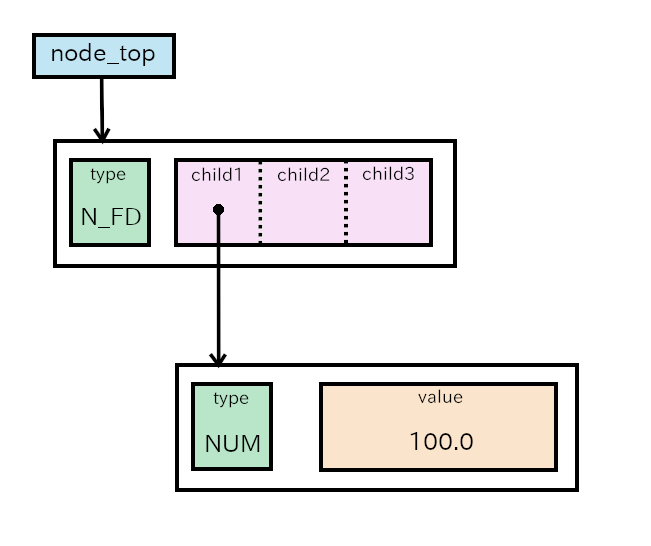
\includegraphics[width=6.51cm,height=5.46cm]{../image/tree.png}
\caption{tree}
\end{figure}

The following is the grammar rule extracted from
\passthrough{\lstinline!turtle.y!}. The rules there are based on the
same idea above. I don't want to explain the whole rules below. Please
look into each line carefully so that you will understand all the rules
and actions.

\begin{lstlisting}
program:
  statement { node_top = $$ = $1; }
| program statement {
        node_top = $$ = tree1 (N_program, $1, $2, NULL);
#ifdef debug
if (node_top == NULL) g_printerr ("program: node_top is NULL.\n"); else g_printerr ("program: node_top is NOT NULL.\n");
#endif
        }
;

statement:
  primary_procedure
| procedure_definition
;

primary_procedure:
  PU    { $$ = tree1 (N_PU, NULL, NULL, NULL); }
| PD    { $$ = tree1 (N_PD, NULL, NULL, NULL); }
| PW expression    { $$ = tree1 (N_PW, $2, NULL, NULL); }
| FD expression    { $$ = tree1 (N_FD, $2, NULL, NULL); }
| TR expression    { $$ = tree1 (N_TR, $2, NULL, NULL); }
| TL expression    { $$ = tree1 (N_TL, $2, NULL, NULL); } /* ver 0.5 */
| BC '(' expression ',' expression ',' expression ')' { $$ = tree1 (N_BC, $3, $5, $7); }
| FC '(' expression ',' expression ',' expression ')' { $$ = tree1 (N_FC, $3, $5, $7); }
 /* assignment */
| ID '=' expression   { $$ = tree1 (N_ASSIGN, tree3 (N_ID, $1), $3, NULL); }
 /* control flow */
| IF '(' expression ')' '{' primary_procedure_list '}' { $$ = tree1 (N_IF, $3, $6, NULL); }
| RT    { $$ = tree1 (N_RT, NULL, NULL, NULL); }
| RS    { $$ = tree1 (N_RS, NULL, NULL, NULL); }
| RP '(' expression ')' '{' primary_procedure_list '}'    { $$ = tree1 (N_RP, $3, $6, NULL); }
 /* user defined procedure call */
| ID '(' ')'  { $$ = tree1 (N_procedure_call, tree3 (N_ID, $1), NULL, NULL); }
| ID '(' argument_list ')'  { $$ = tree1 (N_procedure_call, tree3 (N_ID, $1), $3, NULL); }
;

procedure_definition:
  DP ID '('  ')' '{' primary_procedure_list '}'  {
         $$ = tree1 (N_procedure_definition, tree3 (N_ID, $2), NULL, $6);
        }
| DP ID '(' parameter_list ')' '{' primary_procedure_list '}'  {
         $$ = tree1 (N_procedure_definition, tree3 (N_ID, $2), $4, $7);
        }
;

parameter_list:
  ID { $$ = tree3 (N_ID, $1); }
| parameter_list ',' ID  { $$ = tree1 (N_parameter_list, $1, tree3 (N_ID, $3), NULL); }
;

argument_list:
  expression
| argument_list ',' expression { $$ = tree1 (N_argument_list, $1, $3, NULL); }
;

primary_procedure_list:
  primary_procedure
| primary_procedure_list primary_procedure {
         $$ = tree1 (N_primary_procedure_list, $1, $2, NULL);
        }
;

expression:
  expression '=' expression { $$ = tree1 (N_EQ, $1, $3, NULL); }
| expression '>' expression { $$ = tree1 (N_GT, $1, $3, NULL); }
| expression '<' expression { $$ = tree1 (N_LT, $1, $3, NULL); }
| expression '+' expression { $$ = tree1 (N_ADD, $1, $3, NULL); }
| expression '-' expression { $$ = tree1 (N_SUB, $1, $3, NULL); }
| expression '*' expression { $$ = tree1 (N_MUL, $1, $3, NULL); }
| expression '/' expression { $$ = tree1 (N_DIV, $1, $3, NULL); }
| '-' expression %prec UMINUS { $$ = tree1 (N_UMINUS, $2, NULL, NULL); }
| '(' expression ')' { $$ = $2; }
| ID    { $$ = tree3 (N_ID, $1); }
| NUM   { $$ = tree2 (N_NUM, $1); }
;
\end{lstlisting}

\subsubsection{Epilogue}\label{epilogue}

The epilogue is written in C language and copied to the parser
implementation file. Generally, you can put anything into the epilogue.
In the case of turtle interpreter, the runtime routine and some other
functions are in the epilogue.

\paragraph{Functions to create tree
nodes}\label{functions-to-create-tree-nodes}

There are three functions, \passthrough{\lstinline!tree1!},
\passthrough{\lstinline!tree2!} and \passthrough{\lstinline!tree3!}.

\begin{itemize}
\tightlist
\item
  \passthrough{\lstinline!tree1!} creates a node and sets the node type
  and pointers to its three children (NULL is possible).
\item
  \passthrough{\lstinline!tree2!} creates a node and sets the node type
  and a value (double).
\item
  \passthrough{\lstinline!tree3!} creates a node and sets the node type
  and a pointer to a string.
\end{itemize}

Each function gets memories first and build a node on them. The memories
are inserted to the list. They will be freed when runtime routine
finishes.

The three functions are called in the actions in the rules section.

\begin{lstlisting}[language=C]
/* Dynamically allocated memories are added to the single list. They will be freed in the finalize function. */
GSList *list = NULL;

node_t *
tree1 (int type, node_t *child1, node_t *child2, node_t *child3) {
  node_t *new_node;

  list = g_slist_prepend (list, g_malloc (sizeof (node_t)));
  new_node = (node_t *) list->data;
  new_node->type = type;
  child1(new_node) = child1;
  child2(new_node) = child2;
  child3(new_node) = child3;
  return new_node;
}

node_t *
tree2 (int type, double value) {
  node_t *new_node;

  list = g_slist_prepend (list, g_malloc (sizeof (node_t)));
  new_node = (node_t *) list->data;
  new_node->type = type;
  value(new_node) = value;
  return new_node;
}

node_t *
tree3 (int type, char *name) {
  node_t *new_node;

  list = g_slist_prepend (list, g_malloc (sizeof (node_t)));
  new_node = (node_t *) list->data;
  new_node->type = type;
  name(new_node) = name;
  return new_node;
}
\end{lstlisting}

\paragraph{Symbol table}\label{symbol-table}

Variables and user defined procedures are registered in the symbol
table. This table is a C array. It should be replaced by better
algorithm and data structure, for example hash, in the future version

\begin{itemize}
\tightlist
\item
  Variables are registered with its name and value.
\item
  Procedures are registered with its name and a pointer to the node of
  the procedure.
\end{itemize}

Therefore the table has the following fields.

\begin{itemize}
\tightlist
\item
  type to identify variable or procedure
\item
  name
\item
  value or pointer to a node
\end{itemize}

\begin{lstlisting}[language=C]
#define MAX_TABLE_SIZE 100
enum {
  PROC,
  VAR
};

struct {
  int type;
  char *name;
  union {
    node_t *node;
    double value;
  } object;
} table[MAX_TABLE_SIZE];
int tp;

void
init_table (void) {
  tp = 0;
}
\end{lstlisting}

The function \passthrough{\lstinline!init\_table!} initializes the
table. This must be called before registrations.

There are five functions to access the table,

\begin{itemize}
\tightlist
\item
  \passthrough{\lstinline!proc\_install!} installs a procedure.
\item
  \passthrough{\lstinline!var\_install!} installs a variable.
\item
  \passthrough{\lstinline!proc\_lookup!} looks up a procedure. If the
  procedure is found, it returns a pointer to the node. Otherwise it
  returns NULL.
\item
  \passthrough{\lstinline!var\_lookup!} looks up a variable. If the
  variable is found, it returns TRUE and sets the pointer (argument) to
  point the value. Otherwise it returns FALSE.
\item
  \passthrough{\lstinline!var\_replace!} replaces the value of a
  variable. If the variable hasn't registered yet, it installs the
  variable.
\end{itemize}

\begin{lstlisting}[language=C]
int
tbl_lookup (int type, char *name) {
  int i;

  if (tp == 0)
    return -1;
  for (i=0; i<tp; ++i)
    if (type == table[i].type && strcmp(name, table[i].name) == 0)
      return i;
  return -1;
}

void
tbl_install (int type, char *name, node_t *node, double value) {
  if (tp >= MAX_TABLE_SIZE)
    runtime_error ("Symbol table overflow.\n");
  else if (tbl_lookup (type, name) >= 0)
    runtime_error ("Name %s is already registered.\n", name);
  else {
    table[tp].type = type;
    table[tp].name = name;
    if (type == PROC)
      table[tp++].object.node = node;
    else
      table[tp++].object.value = value;
  }
}

void
proc_install (char *name, node_t *node) {
  tbl_install (PROC, name, node, 0.0);
}

void
var_install (char *name, double value) {
  tbl_install (VAR, name, NULL, value);
}

void
var_replace (char *name, double value) {
  int i;
  if ((i = tbl_lookup (VAR, name)) >= 0)
    table[i].object.value = value;
  else
    var_install (name, value);
}

node_t *
proc_lookup (char *name) {
  int i;
  if ((i = tbl_lookup (PROC, name)) < 0)
    return NULL;
  else
    return table[i].object.node;
}

gboolean
var_lookup (char *name, double *value) {
  int i;
  if ((i = tbl_lookup (VAR, name)) < 0)
    return FALSE;
  else {
    *value = table[i].object.value;
    return TRUE;
  }
}
\end{lstlisting}

\paragraph{Stack for parameters and
arguments}\label{stack-for-parameters-and-arguments}

Stack is a last-in first-out data structure. It is shortened to LIFO.
Turtle uses a stack to keep parameters and arguments. They are like
\passthrough{\lstinline!auto!} class variables in C language. They are
pushed to the stack whenever the procedure is called. LIFO structure is
useful for recursive calls.

Each element of the stack has name and value.

\begin{lstlisting}[language=C]
#define MAX_STACK_SIZE 500
struct {
  char *name;
  double value;
} stack[MAX_STACK_SIZE];
int sp, sp_biggest;

void
init_stack (void) {
  sp = sp_biggest = 0;
}
\end{lstlisting}

\passthrough{\lstinline!sp!} is a stack pointer. It is an index of the
array \passthrough{\lstinline!stack!} and it always points an element of
the array to store the next data. \passthrough{\lstinline!sp\_biggest!}
is the biggest number assigned to \passthrough{\lstinline!sp!}. We can
know the amount of elements used in the array during the runtime. The
purpose of the variable is to find appropriate
\passthrough{\lstinline!MAX\_STACK\_SIZE!}. It will be unnecessary in
the future version if the stack is implemented with better data
structure and memory allocation.

The runtime routine push data to the stack when it executes a node of a
procedure call. (The type of the node is
\passthrough{\lstinline!N\_procedure\_call!}.)

\begin{lstlisting}
dp drawline (angle, distance) { ... ... ... }
drawline (90, 100)
\end{lstlisting}

\begin{itemize}
\tightlist
\item
  The first line defines a procedure \passthrough{\lstinline!drawline!}.
  The runtime routine stores the name \passthrough{\lstinline!drawline!}
  and the node of the procedure to the symbol table.
\item
  The second line calls the procedure. First, it looks for the procedure
  in the symbol table and gets its node. Then it searches the node for
  the parameters and gets \passthrough{\lstinline!angle!} and
  \passthrough{\lstinline!distance!}.
\item
  It pushes (``angle'', 90.0) to the stack.
\item
  It pushes (``distance'', 100.0) to the stack.
\item
  It pushes (NULL, 2.0) to the stack. The number 2.0 is the number of
  parameters (or arguments). It is used when the procedure returns.
\end{itemize}

The following diagram shows the structure of the stack. First,
\passthrough{\lstinline!procedure 1!} is called. The procedure has two
parameters. In the \passthrough{\lstinline!procedure 1!}, another
procedure \passthrough{\lstinline!procedure 2!} is called. It has one
parameter. In the \passthrough{\lstinline!procedure 2!}, another
procedure \passthrough{\lstinline!procedure 3!} is called. It has three
parameters. These three procedures are nested.

Programs push data to a stack from a low address memory to a high
address memory. In the following diagram, the lowest address is at the
top and the highest address is at the bottom. That is the order of the
address. However, ``the top of the stack'' is the last pushed data and
``the bottom of the stack'' is the first pushed data. Therefore, ``the
top of the stack'' is the bottom of the rectangle in the diagram and
``the bottom of the stack'' is the top of the rectangle.

\begin{figure}
\centering
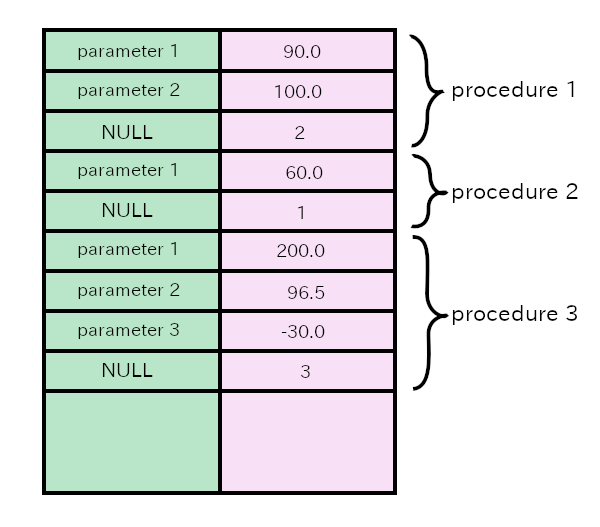
\includegraphics[width=6.64cm,height=8.05cm]{../image/stack.png}
\caption{Stack}
\end{figure}

There are four functions to access the stack.

\begin{itemize}
\tightlist
\item
  \passthrough{\lstinline!stack\_push!} pushes data to the stack.
\item
  \passthrough{\lstinline!stack\_lookup!} searches the stack for the
  variable given its name as an argument. It searches only the
  parameters of the latest procedure. It returns TRUE and sets the
  argument \passthrough{\lstinline!value!} to point the value, if the
  variable has been found. Otherwise it returns FALSE.
\item
  \passthrough{\lstinline!stack\_replace!} replaces the value of the
  variable in the stack. If it succeeds, it returns TRUE. Otherwise
  returns FALSE.
\item
  \passthrough{\lstinline!stack\_return!} throws away the latest
  parameters. The stack pointer goes back to the point before the latest
  procedure call so that it points to parameters of the previous called
  procedure.
\end{itemize}

\begin{lstlisting}[language=C]
void
stack_push (char *name, double value) {
  if (sp >= MAX_STACK_SIZE)
    runtime_error ("Stack overflow.\n");
  else {
    stack[sp].name = name;
    stack[sp++].value = value;
    sp_biggest = sp > sp_biggest ? sp : sp_biggest;
  }
}

int
stack_search (char *name) {
  int depth, i;

  if (sp == 0)
    return -1;
  depth = (int) stack[sp-1].value;
  if (depth + 1 > sp) /* something strange */
    runtime_error ("Stack error.\n");
  for (i=0; i<depth; ++i)
    if (strcmp(name, stack[sp-(i+2)].name) == 0) {
      return sp-(i+2);
    }
  return -1;
}

gboolean
stack_lookup (char *name, double *value) {
  int i;

  if ((i = stack_search (name)) < 0)
    return FALSE;
  else {
    *value = stack[i].value;
    return TRUE;
  }
}

gboolean
stack_replace (char *name, double value) {
  int i;

  if ((i = stack_search (name)) < 0)
    return FALSE;
  else {
    stack[i].value = value;
    return TRUE;
  }
}

void
stack_return(void) {
  int depth;

  if (sp <= 0)
    return;
  depth = (int) stack[sp-1].value;
  if (depth + 1 > sp) /* something strange */
    runtime_error ("Stack error.\n");
  sp -= depth + 1;
}
\end{lstlisting}

\paragraph{Surface and cairo}\label{surface-and-cairo}

A global variable \passthrough{\lstinline!surface!} is shared by
\passthrough{\lstinline!turtleapplication.c!} and
\passthrough{\lstinline!turtle.y!}. It is initialized in
\passthrough{\lstinline!turtleapplication.c!}.

The runtime routine has its own cairo context. This is different from
the cairo in the GtkDrawingArea instance. The runtime routine draws a
shape on the \passthrough{\lstinline!surface!} with the cairo context.
After runtime routine returns to \passthrough{\lstinline!run\_cb!},
\passthrough{\lstinline!run\_cb!} adds the GtkDrawingArea widget to the
queue to redraw. When the widget is redraw,the drawing function
\passthrough{\lstinline!draw\_func!} is called. It copies the
\passthrough{\lstinline!surface!} to the surface in the GtkDrawingArea
object.

\passthrough{\lstinline!turtle.y!} has two functions
\passthrough{\lstinline!init\_cairo!} and
\passthrough{\lstinline!destroy\_cairo!}.

\begin{itemize}
\tightlist
\item
  \passthrough{\lstinline!init\_cairo!} initializes static variables and
  cairo context. The variables keep pen status (up or down), direction,
  initial location, line width and color. The size of the
  \passthrough{\lstinline!surface!} changes according to the size of the
  window. Whenever a user drags and resizes the window, the
  \passthrough{\lstinline!surface!} is also resized.
  \passthrough{\lstinline!init\_cairo!} gets the size first and sets the
  initial location of the turtle (center of the surface) and the
  transformation matrix.
\item
  \passthrough{\lstinline!destroy\_cairo!} just destroys the cairo
  context.
\end{itemize}

Turtle has its own coordinate. The origin is at the center of the
surface, and positive direction of x and y axes are right and up
respectively. But surfaces have its own coordinate. Its origin is at the
top-left corner of the surface and positive direction of x and y are
right and down respectively. A plane with the turtle's coordinate is
called user space, which is the same as cairo's user space. A plane with
the surface's coordinate is called device space.

Cairo provides a transformation which is an affine transformation. It
transforms a user-space coordinate (x, y) into a device-space coordinate
(z, w).

\begin{figure}
\centering
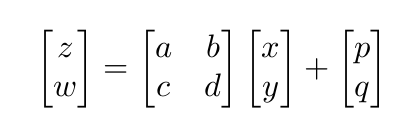
\includegraphics[width=6.3cm,height=2.04cm]{../image/transformation.png}
\caption{transformation}
\end{figure}

The function \passthrough{\lstinline!init\_cairo!} gets the width and
height of the \passthrough{\lstinline!surface!} (See the program below).

\begin{itemize}
\tightlist
\item
  The center of the surface is (0,0) with regard to the user-space
  coordinate and (width/2, height/2) with regard to the device-space
  coordinate.
\item
  The positive direction of x axis in the two spaces are the same. So,
  (1,0) is transformed into (1+width/2,height/2).
\item
  The positive direction of y axis in the two spaces are opposite. So,
  (0,1) is transformed into (width/2,-1+height/2).
\end{itemize}

You can determine a, b, c, d, p and q by substituting the numbers above
for x, y, z and w in the equation above. The solution of the
simultaneous equations is:

\begin{lstlisting}
a = 1, b = 0, c = 0, d = -1, p = width/2, q = height/2
\end{lstlisting}

Cairo provides a structure \passthrough{\lstinline!cairo\_matrix\_t!}.
The function \passthrough{\lstinline!init\_cairo!} uses it and sets the
cairo transformation (See the program below). Once the matrix is set,
the transformation always performs whenever
\passthrough{\lstinline!cairo\_stroke!} function is invoked.

\begin{lstlisting}[language=C]
/* status of the surface */
static gboolean pen = TRUE;
static double angle = 90.0; /* angle starts from x axis and measured counterclockwise */
                   /* Initially facing to the north */
static double cur_x = 0.0;
static double cur_y = 0.0;
static double line_width = 2.0;

struct color {
  double red;
  double green;
  double blue;
};
static struct color bc = {0.95, 0.95, 0.95}; /* white */
static struct color fc = {0.0, 0.0, 0.0}; /* black */

/* cairo */
static cairo_t *cr;
gboolean
init_cairo (void) {
  int width, height;
  cairo_matrix_t matrix;

  pen = TRUE;
  angle = 90.0;
  cur_x = 0.0;
  cur_y = 0.0;
  line_width = 2.0;
  bc.red = 0.95; bc.green = 0.95; bc.blue = 0.95;
  fc.red = 0.0; fc.green = 0.0; fc.blue = 0.0;

  if (surface) {
    width = cairo_image_surface_get_width (surface);
    height = cairo_image_surface_get_height (surface);
    matrix.xx = 1.0; matrix.xy = 0.0; matrix.x0 = (double) width / 2.0;
    matrix.yx = 0.0; matrix.yy = -1.0; matrix.y0 = (double) height / 2.0;

    cr = cairo_create (surface);
    cairo_transform (cr, &matrix);
    cairo_set_source_rgb (cr, bc.red, bc.green, bc.blue);
    cairo_paint (cr);
    cairo_set_source_rgb (cr, fc.red, fc.green, fc.blue);
    cairo_move_to (cr, cur_x, cur_y);
    return TRUE;
  } else
    return FALSE;
}

void
destroy_cairo () {
  cairo_destroy (cr);
}
\end{lstlisting}

\paragraph{Eval function}\label{eval-function}

A function \passthrough{\lstinline!eval!} evaluates an expression and
returns the value of the expression. It calls itself recursively. For
example, if the node is \passthrough{\lstinline!N\_ADD!}, then:

\begin{enumerate}
\def\labelenumi{\arabic{enumi}.}
\tightlist
\item
  Calls eval(child1(node)) and gets the value1.
\item
  Calls eval(child2(node)) and gets the value2.
\item
  Returns value1+value2.
\end{enumerate}

This is performed by a macro \passthrough{\lstinline!calc!} defined in
the sixth line in the following program.

\begin{lstlisting}[language=C]
double
eval (node_t *node) {
double value = 0.0;
  if (node == NULL)
    runtime_error ("No expression to evaluate.\n");
#define calc(op) eval (child1(node)) op eval (child2(node))
  switch (node->type) {
    case N_EQ:
      value = (double) calc(==);
      break;
    case N_GT:
      value = (double) calc(>);
      break;
    case N_LT:
      value = (double) calc(<);
      break;
    case N_ADD:
      value = calc(+);
      break;
    case N_SUB:
      value = calc(-);
      break;
    case N_MUL:
      value = calc(*);
      break;
    case N_DIV:
      if (eval (child2(node)) == 0.0)
        runtime_error ("Division by zerp.\n");
      else
        value = calc(/);
      break;
    case N_UMINUS:
      value = -(eval (child1(node)));
      break;
    case N_ID:
      if (! (stack_lookup (name(node), &value)) && ! var_lookup (name(node), &value) )
        runtime_error ("Variable %s not defined.\n", name(node));
      break;
    case N_NUM:
      value = value(node);
      break;
    default:
      runtime_error ("Illegal expression.\n");
  }
  return value;
}
\end{lstlisting}

\paragraph{Execute function}\label{execute-function}

Primary procedures and procedure definitions are analyzed and executed
by the function \passthrough{\lstinline!execute!}. It doesn't return any
values. It calls itself recursively. The process of
\passthrough{\lstinline!N\_RT!} and
\passthrough{\lstinline!N\_procedure\_call!} is complicated. It will
explained after the following program. Other parts are not so difficult.
Read the program below carefully so that you will understand the
process.

\begin{lstlisting}[language=C]
/* procedure - return status */
static int proc_level = 0;
static int ret_level = 0;

void
execute (node_t *node) {
  double d, x, y;
  char *name;
  int n, i;

  if (node == NULL)
    runtime_error ("Node is NULL.\n");
  if (proc_level > ret_level)
    return;
  switch (node->type) {
    case N_program:
      execute (child1(node));
      execute (child2(node));
      break;
    case N_PU:
      pen = FALSE;
      break;
    case N_PD:
      pen = TRUE;
      break;
    case N_PW:
      line_width = eval (child1(node)); /* line width */
      break;
    case N_FD:
      d = eval (child1(node)); /* distance */
      x = d * cos (angle*M_PI/180);
      y = d * sin (angle*M_PI/180);
      /* initialize the current point = start point of the line */
      cairo_move_to (cr, cur_x, cur_y);
      cur_x += x;
      cur_y += y;
      cairo_set_line_width (cr, line_width);
      cairo_set_source_rgb (cr, fc.red, fc.green, fc.blue);
      if (pen)
        cairo_line_to (cr, cur_x, cur_y);
      else
        cairo_move_to (cr, cur_x, cur_y);
      cairo_stroke (cr);
      break;
    case N_TR:
      angle -= eval (child1(node));
      for (; angle < 0; angle += 360.0);
      for (; angle>360; angle -= 360.0);
      break;
    case N_BC:
      bc.red = eval (child1(node));
      bc.green = eval (child2(node));
      bc.blue = eval (child3(node));
#define fixcolor(c)  c = c < 0 ? 0 : (c > 1 ? 1 : c)
      fixcolor (bc.red);
      fixcolor (bc.green);
      fixcolor (bc.blue);
      /* clear the shapes and set the background color */
      cairo_set_source_rgb (cr, bc.red, bc.green, bc.blue);
      cairo_paint (cr);
      break;
    case N_FC:
      fc.red = eval (child1(node));
      fc.green = eval (child2(node));
      fc.blue = eval (child3(node));
      fixcolor (fc.red);
      fixcolor (fc.green);
      fixcolor (fc.blue);
      break;
    case N_ASSIGN:
      name = name(child1(node));
      d = eval (child2(node));
      if (! stack_replace (name, d)) /* First, tries to replace the value in the stack (parameter).*/
        var_replace (name, d); /* If the above fails, tries to replace the value in the table. If the variable isn't in the table, installs it, */
      break;
    case N_IF:
      if (eval (child1(node)))
        execute (child2(node));
      break;
    case N_RT:
      ret_level--;
      break;
    case N_RS:
      pen = TRUE;
      angle = 90.0;
      cur_x = 0.0;
      cur_y = 0.0;
      line_width = 2.0;
      fc.red = 0.0; fc.green = 0.0; fc.blue = 0.0;
      /* To change background color, use bc. */
      break;
    case N_procedure_call:
      name = name(child1(node));
node_t *proc = proc_lookup (name);
      if (! proc)
        runtime_error ("Procedure %s not defined.\n", name);
      if (strcmp (name, name(child1(proc))) != 0)
        runtime_error ("Unexpected error. Procedure %s is called, but invoked procedure is %s.\n", name, name(child1(proc)));
/* make tuples (parameter (name), argument (value)) and push them to the stack */
node_t *param_list;
node_t *arg_list;
      param_list = child2(proc);
      arg_list = child2(node);
      if (param_list == NULL) {
        if (arg_list == NULL) {
          stack_push (NULL, 0.0); /* number of argument == 0 */
        } else
          runtime_error ("Procedure %s has different number of argument and parameter.\n", name);
      }else {
/* Don't change the stack until finish evaluating the arguments. */
#define TEMP_STACK_SIZE 20
        char *temp_param[TEMP_STACK_SIZE];
        double temp_arg[TEMP_STACK_SIZE];
        n = 0;
        for (; param_list->type == N_parameter_list; param_list = child1(param_list)) {
          if (arg_list->type != N_argument_list)
            runtime_error ("Procedure %s has different number of argument and parameter.\n", name);
          if (n >= TEMP_STACK_SIZE)
            runtime_error ("Too many parameters. the number must be %d or less.\n", TEMP_STACK_SIZE);
          temp_param[n] = name(child2(param_list));
          temp_arg[n] = eval (child2(arg_list));
          arg_list = child1(arg_list);
          ++n;
        }
        if (param_list->type == N_ID && arg_list -> type != N_argument_list) {
          temp_param[n] = name(param_list);
          temp_arg[n] = eval (arg_list);
          if (++n >= TEMP_STACK_SIZE)
            runtime_error ("Too many parameters. the number must be %d or less.\n", TEMP_STACK_SIZE);
          temp_param[n] = NULL;
          temp_arg[n] = (double) n;
          ++n;
        } else
          runtime_error ("Unexpected error.\n");
        for (i = 0; i < n; ++i)
          stack_push (temp_param[i], temp_arg[i]);
      }
      ret_level = ++proc_level;
      execute (child3(proc));
      ret_level = --proc_level;
      stack_return ();
      break;
    case N_procedure_definition:
      name = name(child1(node));
      proc_install (name, node);
      break;
    case N_primary_procedure_list:
      execute (child1(node));
      execute (child2(node));
      break;
    default:
      runtime_error ("Unknown statement.\n");
  }
}
\end{lstlisting}

A node \passthrough{\lstinline!N\_procedure\_call!} is created by the
parser when it has found a user defined procedure call. The procedure
has been defined in the prior statement. Suppose the parser reads the
following example code.

\begin{lstlisting}
dp drawline (angle, distance) {
  tr angle
  fd distance
}
drawline (90, 100)
drawline (90, 100)
drawline (90, 100)
drawline (90, 100)
\end{lstlisting}

This example draws a square.

When The parser reads the lines from one to four, it creates nodes like
this:

\begin{figure}
\centering
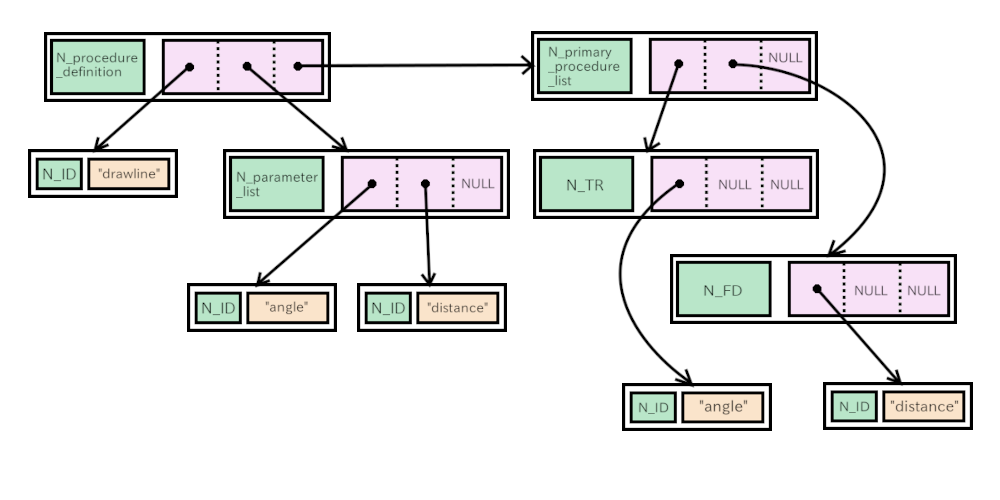
\includegraphics[width=10cm,height=6cm]{../image/tree2.png}
\caption{Nodes of drawline}
\end{figure}

Runtime routine just stores the procedure to the symbol table with its
name and node.

\begin{figure}
\centering
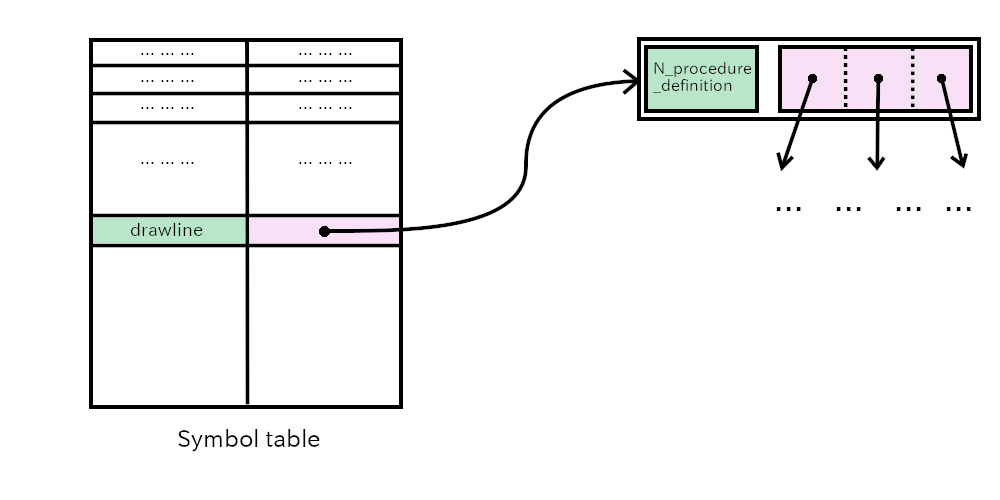
\includegraphics[width=10cm,height=5cm]{../image/table.png}
\caption{Symbol table}
\end{figure}

When the parser reads the fifth line in the example, it creates nodes
like this:

\begin{figure}
\centering
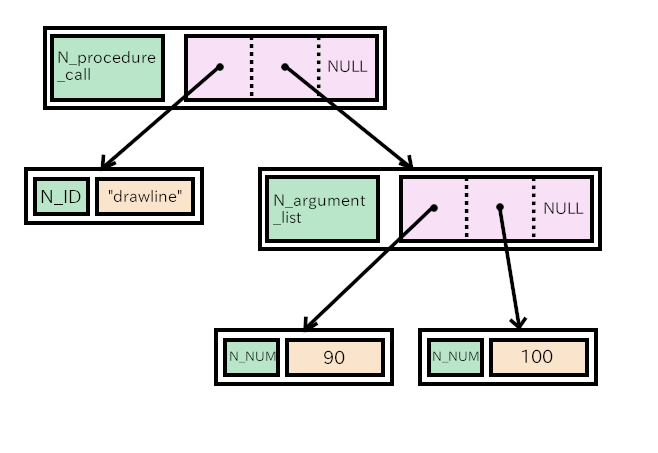
\includegraphics[width=10cm,height=5cm]{../image/proc_call.png}
\caption{Nodes of procedure call}
\end{figure}

When the runtime routine meets
\passthrough{\lstinline!N\_procedure\_call!} node, it behaves like this:

\begin{enumerate}
\def\labelenumi{\arabic{enumi}.}
\tightlist
\item
  Searches the symbol table for the procedure with the name.
\item
  Gets pointers to the node to parameters and the node to the body.
\item
  Creates a temporary stack. Makes a tuple of each parameter name and
  argument value. Pushes the tuples into the stack, and (NULL, number of
  parameters) finally. If no error occurs, copies them from the
  temporary stack to the parameter stack.
\item
  Increases \passthrough{\lstinline!prc\_level!} by one. Sets
  \passthrough{\lstinline!ret\_level!} to the same value as
  \passthrough{\lstinline!proc\_level!}.
  \passthrough{\lstinline!proc\_level!} is zero when runtime routine
  runs on the main routine. If it goes into a procedure,
  \passthrough{\lstinline!proc\_level!} increases by one. Therefore,
  \passthrough{\lstinline!proc\_level!} is the depth of the procedure
  call. \passthrough{\lstinline!ret\_level!} is the level to return. If
  it is the same as \passthrough{\lstinline!proc\_level!}, runtime
  routine executes commands in order of the commands in the procedure.
  If it is smaller than \passthrough{\lstinline!proc\_level!}, runtime
  routine doesn't execute commands until it becomes the same level as
  \passthrough{\lstinline!proc\_level!}.
  \passthrough{\lstinline!ret\_level!} is used to return the procedure.
\item
  Executes the node of the body of the procedure.
\item
  Decreases \passthrough{\lstinline!proc\_level!} by one. Sets
  \passthrough{\lstinline!ret\_level!} to the same value as
  \passthrough{\lstinline!proc\_level!}. Calls
  \passthrough{\lstinline!stack\_return!}.
\end{enumerate}

When the runtime routine meets \passthrough{\lstinline!N\_RT!} node, it
decreases \passthrough{\lstinline!ret\_level!} by one so that the
following commands in the procedure are ignored by the runtime routine.

\paragraph{Runtime entry and error
functions}\label{runtime-entry-and-error-functions}

A function \passthrough{\lstinline!run!} is the entry of the runtime
routine. A function \passthrough{\lstinline!runtime\_error!} reports an
error occurred during the runtime routine runs. (Errors which occur
during the parsing are called syntax error and reported by
\passthrough{\lstinline!yyerror!}.) After
\passthrough{\lstinline!runtime\_error!} reports an error, it stops the
command execution and goes back to \passthrough{\lstinline!run!} to
exit.

Setjmp and longjmp functions are used. They are declared in
\passthrough{\lstinline!<setjmp.h>!}.
\passthrough{\lstinline!setjmp (buf)!} saves state information in
\passthrough{\lstinline!buf!} and returns zero.
\passthrough{\lstinline!longjmp(buf, 1)!} restores the state information
from \passthrough{\lstinline!buf!} and returns
\passthrough{\lstinline!1!} (the second argument). Because the
information is the status at the time \passthrough{\lstinline!setjmp!}
is called, so longjmp resumes the execution at the next of setjmp
function call. In the following program, longjmp resumes at the
assignment to the variable \passthrough{\lstinline!i!}. When setjmp is
called, 0 is assigned to \passthrough{\lstinline!i!} and
\passthrough{\lstinline!execute(node\_top)!} is called. On the other
hand, when longjmp is called, 1 is assigned to
\passthrough{\lstinline!i!} and
\passthrough{\lstinline!execute(node\_top)!} is not called..

\passthrough{\lstinline!g\_slist\_free\_full!} frees all the allocated
memories.

\begin{lstlisting}[language=C]
static jmp_buf buf;

void
run (void) {
  int i;

  if (! init_cairo()) {
    g_print ("Cairo not initialized.\n");
    return;
  }
  init_table();
  init_stack();
  ret_level = proc_level = 1;
  i = setjmp (buf);
  if (i == 0)
    execute(node_top);
  /* else ... get here by calling longjmp */
  destroy_cairo ();
  g_slist_free_full (g_steal_pointer (&list), g_free);
}

/* format supports only %s, %f and %d */
static void
runtime_error (char *format, ...) {
  va_list args;
  char *f;
  char b[3];
  char *s;
  double v;
  int i;

  va_start (args, format);
  for (f = format; *f; f++) {
    if (*f != '%') {
      b[0] = *f;
      b[1] = '\0';
      g_print ("%s", b);
      continue;
    }
    switch (*++f) {
      case 's':
        s = va_arg(args, char *);
        g_print ("%s", s);
        break;
      case 'f':
        v = va_arg(args, double);
        g_print("%f", v);
        break;
      case 'd':
        i = va_arg(args, int);
        g_print("%d", i);
        break;
      default:
        b[0] = '%';
        b[1] = *f;
        b[2] = '\0';
        g_print ("%s", b);
        break;
    }
  }
  va_end (args);

  longjmp (buf, 1);
}
\end{lstlisting}

A function \passthrough{\lstinline!runtime\_error!} has a
variable-length argument list.

\begin{lstlisting}[language=C]
void runtime_error (char *format, ...)
\end{lstlisting}

This is implemented with \passthrough{\lstinline!<stdarg.h>!} header
file. The \passthrough{\lstinline!va\_list!} type variable
\passthrough{\lstinline!args!} will refer to each argument in turn. A
function \passthrough{\lstinline!va\_start!} initializes
\passthrough{\lstinline!args!}. A function
\passthrough{\lstinline!va\_arg!} returns an argument and moves the
reference of \passthrough{\lstinline!args!} to the next. A function
\passthrough{\lstinline!va\_end!} cleans up everything necessary at the
end.

The function \passthrough{\lstinline!runtime\_error!} has a similar
format of printf standard function. But its format has only
\passthrough{\lstinline!\%s!}, \passthrough{\lstinline!\%f!} and
\passthrough{\lstinline!\%d!}.

The functions declared in \passthrough{\lstinline!<setjmp.h>!} and
\passthrough{\lstinline!<stdarg.h>!} are explained in the very famous
book ``The C programming language'' written by Brian Kernighan and
Dennis Ritchie. I referred to the book to write the program above.

The program \passthrough{\lstinline!turtle!} is unsophisticated and
unpolished. If you want to make your own language, you need to know more
and more. I don't know any good textbook about compilers and
interpreters. If you know a good book, please let me know.

However, the following information is very useful (but old).

\begin{itemize}
\tightlist
\item
  Bison documentation
\item
  Flex documentation
\item
  Software tools written by Brian W. Kernighan \& P. J. Plauger (1976)
\item
  Unix programming environment written by Brian W. Kernighan and Rob
  Pike (1984)
\item
  Source code of a language, for example, ruby.
\end{itemize}

Lately, lots of source codes are in the internet. Maybe reading source
codes is the most useful for programmers.
